\def\stmt{$A$}
% \def\stmt{$\phi$}


\commentout{%oli-v1
	The ability to articulate a \emph{degree of confidence} 
	% (or the opposite: a degree of uncertainty)
	is a critical aspect of representing knowledge.
	There are 
	many well-established ways to quantify (un)certinaty \parencite[\S2]{halpern2017reasoning},
		and chief among them is probability.
	While ``confidence'' can be coherently read in probabilistic terms,
		such usage may shadow another important concept.
	This paper details a different conception that arises when updating beliefs. 
	As we shall see, this notion of confidence
	complements traditional representations of uncertainty (such as probability), 
	and moreover unifies several different concepts across AI.
}

What should it mean to say that one has a high degree of confidence in a statement $\phi$?  It is often taken to mean that we think $\phi$ is likely. 
% This paper details a different conception that arises when updating beliefs. 
% As we shall see, this notion of confidence
% complements traditional representations of uncertainty (such as probability), 
Here we argue that there is a related but more useful conception of confidence that arises when learning---one that complements likelihood and, moreover, unifies several different concepts in the literature.
% Here we argue that there is a related but more useful way of defining confidence, which complements notions like probability and, moreover, unifies several different concepts in the literature.

For us, confidence is a measure of \emph{trust}, rather than likelihood.
In particular, the {degree of confidence} that one has in a piece of information $\phi$
%is a number  $\chi \in [\bot,\top]$ that 
quantifies how seriously to take $\phi$ in updating one's beliefs. 
So at one extreme,
if we observe $\phi$ but have no confidence in it, 
we should not change our beliefs at all;
at the other, if we have full confidence in $\phi$,
 we should fully incorporate it into our beliefs.

% If our belief state is a probability measure $\Pr$ and $\phi$ is an event, for example, then fully incorporating $\phi$ amounts to conditioning $\Pr$ on it.
\begin{example} \label{ex:prob-simple}
Suppose our belief state is a probability measure, and $\phi$ is an event. 
A full-confidence update then amounts to conditioning on $\phi$, after which $\phi$ has probability 1, and so cannot be further incorporated.
%oli1: changed from "the obvious way" to "an obvious way"
% In a probabilistic setting, we can capture an  intermediate degree of confidence by interpolating in the obvious way:
% In this case,
% we can also capture intermediate degrees of confidence in an obvious way:
%oli2:
% We also have an obvious way
Here is an obvious way
to describe intermediate degrees of confidence:
if we learn $\phi$ with confidence
%oli1: now adding range here
% $\alpha$
$\alpha \in [0,1]$
% and start with a prior probability $\Pr$, then we end up with the
and start with prior probability $\Pr$, then we end up with the
%oli1: I agree that this notation is nicer, but these days it
% is also much less standard than p(X) and p(X|\phi). In particular,
% my ML friends who work with applied probability a lot do not understand
% how to parse  "\Pr | \phi". 
posterior $(1-\alpha)\Pr + \alpha (\Pr\mid \phi)$.
%
Thus, having high confidence in $\phi$ leads to posterior beliefs that give $\phi$
high probability.
The converse is false, however, so
confidence and probability can be quite different.
% 
%oli1: the context here has been stripped; we're now missing how it might be possible to learn \phi with low confidence if we already assign it high probability.
% If we start out with a prior that gives $\phi$ high likelihood, and learn $\phi$ with low confidence, our posterior beliefs still give $\phi$ high likelihood.  
% We might also have a great deal of confidence in an observation of $\phi$  despite having a low prior belief in $\phi$.
If an untrusted source tells us $\phi$ which we already happen to believe, 
then our prior assigns $\phi$ high probability,
we learn $\phi$ with low confidence,
and our posterior beliefs still give $\phi$ high probability.  
% then we learn $\phi$ with low confidence, but both 
% Confidence is even easier to distinguish from prior probability: 
%joe1: I don't know what "more independent" means
%Confidence and prior probability are even more independent:
% Confidence is even less coupled to prior probability:
Prior probabilty is further decoupled from confidence:
if we learn a surprising fact $\phi$ from a trusted source, we have high confidence in $\phi$ despite it having low prior probability.
% This leads to an important observation: one's confidence in $\phi$ is not a feature of one's prior probability at all.
\end{example}

\commentout{
	In this context, 
	the confidence $\chi \in [0,1]$ has a clear interpretation as the ``fraction of the way towards full incorporation'',
	but in others,
	it may be 
	less clear what a number on this scale (say, $\chi{=}0.7$) means.
	% there is still a natural path from distrust to complete trust that is parameterized differently.
	% In other cases, there are other more natural ways to articulate one's confidence.
}

{\color{red}% now misplaced
In some contexts, both styles of measuring confidence are used. 
To illustrate, 
we turn to another class of examples of confidence
% in a different specialized context.
% This one is 
based on the work of 
\citeauthor{shafer1976mathematical},
whose 
\citeyear{shafer1976mathematical} book
was written largely 
% with our notion of confidence in mind. 
to develop a theory of what we have been calling confidence,
based on (and tailored to) to his preferred representation of
uncertainty. 
% Mathematical Theory of Evidence (\citeyear{shafer1976mathematical},
% purpose was precisely to 
%
% The utility of these two different representations
% of confidence 
% was well-understood by
% \textcite{shafer1976mathematical}.
}

\begin{example} \label{ex:shafer}
Let $W$ be a finite set of possible worlds, 
and suppose our belief state is a 
% generalization of a probability over $W$ called a
% Dempster-Shafer belief function, 
% % which is a particular generalization of a finite probability measure,
% % $\Bel : 2^W \to [0,1]$ which intuitively assigns each subset of $W$ 
% % a degree of belief
% or equivalently, a
% \emph{basic probability assignment}: a function $m : 2^W \to [0,1]$
\emph{mass function} $m : 2^W \! \to\! [0,1]$
satisfying $\sum_{U \subseteq W} m(U) \!=\! 1$ 
and $m(\emptyset) \!=\! 0$. 
% The belief function corresponding to $m$ assigns belief
% This correponds to a belief function by
From $m$, one can obtain 
a Dempster-Shafer belief function, 
which is a generalization of a finite probability measure over $W$, by
$\Bel_m(U) = \sum_{V \subseteq U} m(V)$
\parencite{shafer1976mathematical}.
%

Suppose we come accross evidence that supports an event $\phi 
\subseteq W$ to a degree $\alpha \in [0,1]$.
Together, $\phi$ and our confidence $\alpha$ in it
can be represented by another mass function $s$,
called a \emph{simple support function},
% that assigns $s(\phi) = \alpha$, $s(W) = 1-\alpha$ and $s(U) = 0$ for all other $U \subseteq W$.
% Intuitively, $s$ supports $\phi$ to degree $\alpha$, but otherwise
% says nothing, since it places the rest of its mass on the trivial event.
that places $\alpha$ of its mass on $\phi$, and the rest on the trivial event $W$.
% a second basic probability assignment $s = \alpha\, A + (1-\alpha)\,  W$
% a second mass function $s = \alpha\, \phi + (1-\alpha)\,  W$
% (that is, $s(A) = \alpha$, $s(W) = 1-\alpha$, and $s(U) = 0$ for all other $U \subseteq W$)
%
% a belief function
% \[
% 	S(U) = \begin{cases}
% 	0 &\text{ if } U \subsetneq A \\
% 	\alpha &\text{ if } A \subseteq U  \subsetneq W; \\
% 	1 &\text{ if } U = W.	
% \end{cases}
% \]
%
To combine our prior belief $m$ with the new evidence $s$,
Shafer argues we should use Dempster's rule of combination,
% to obtain a posterior belief
to obtain a posterior $m' := m \oplus s$, 
given in this case by:
% which in this case equals
% a complicated-looking
% posterior 
% $m'$ whose value at each 
% % $\emptyset \ne$
% non-empty $B \subseteq W$ is:
 % $m'$ by:
% $ m'(B) := $
\begin{align*}
	% m' &:= m \oplus s \\[-1ex]
	% m'(U) &:= (m \oplus s)(U) \\[-0.5ex]
 	m'(U) &= 
	% =U &\mapsto
	% =\;&
	% &
	% \frac{1}{1\!-\!k} 
	% \sum_{\substack{U,V \mathrlap{\subseteq W} \\ U \cap V \mathrlap{= B}}}
	% 		m(U) s_{\!A}(V), ~~
	% \text{where}~~
	% k := \sum_{\mathclap{\substack{U,V \subseteq W \\ U \cap V = \emptyset}}}
	%  	m(u) s_{\!A}(V)
	% \\
	% %
	% &= 
	\frac{1}{\!\displaystyle 1 - \alpha \sum_{\mathclap{V \subseteq (W \setminus \phi)}} m(V)\!}
	\Big(
	(1-\alpha) m(U) + 
	\alpha \sum_{\substack{\mathclap{V \subseteq W} \\ \mathllap{V \cap \phi} = \mathrlap{U}}} m(V) 
		\Big).
\end{align*}
It is easy to verify that when $\alpha = 0$, the posterior beliefs are the same as the
prior ones, and that when $\alpha = 1$,
 % this has the effect of removing all 
% one effect is to discard the mass from sets
all mass is assigned to subsets of $\phi$.
It follows that, after the update, $\Bel_{m'}(\phi)$.
% It follows that the posterior degree of belief 
% in $\phi$, (or any set that contains $\phi$) equals one.
So again, we have two extremes in confidence, continuously parameterized
by a value $\alpha \in [0,1]$.
% equals $1$ for every $U$ that contains $A$.
% $W$ that are not subsets of $A$
% so that now $\Bel_{m'}(B) = 1$ for all $B \supseteq A$. 
% \[
% 	m'(B) =\begin{cases}
% 		& \text{ if } B \subseteq A \\
% 		& \text{otherwise}
% 	\end{cases}
% \]

% What if $m$ itself is a simple support function on $A$?
% When combining two simple support functions both on $A$, we might
% want to describe 
We now look at some special cases. Suppose that $\Bel_m$ is a probability 
measure $\Pr$, or equivalently, that $m$ only assigns mass to singletons.
% measure, meaning that gives mass only to singletons, then $m'$ is as well,
% measure $p$, meaning that $m(\{x\}) = p(\{x\})$ and $m(U) = 0$ when $U$ is not a singleton, then
% $m'$ is also a probability measure, and is given by:
Then $m'$ also only assigns mass to singletons, and is given by:
\begin{equation}
m'(\{x\}) =
 % \frac{\alpha \mathbbm1[x \in A] p(x) + (1-\alpha) p(x)}{1 - \alpha + \alpha p(A)}.
 % \frac{\alpha\; m(\{x\} \cap A) + (1-\alpha)\, m(\{x\})}{1 - \alpha + \alpha\; \sum_{y \in A} m(\{y\})}.
 % \frac{\alpha\; (\{x\} \cap A) + (1-\alpha)\, p(\{x\})}{1 - \alpha + \alpha\; p(A)}.
 \frac{\alpha\; \Pr(\{x\} \cap \phi) + (1-\alpha)\, \Pr(\{x\})}{1 - \alpha + \alpha\; \Pr(\phi)}.
 	\label{eq:ds-prob}
\end{equation}
Thus, as a function of $\alpha \in [0,1]$, $m'$ is  
% a path that begins at $p$ and ends at $p|A$,
a path that begins at $\Pr$,  ends at $(\Pr |\phi)$,
and can even be viewed as a ``proportion of the way to incorporation'',
just like in \cref{ex:prob-simple}---yet it is parameterized differently.
% Thus, we need more assumptions in order to pin down the exact meaning of an intermediate confidence value.
Therefore, to appropriately determine a numerical value of confidence, you need
to know something more about the updating procedure. 
% In \cref{sec:loss-repr}, we will
% develop tools we need to fully understand the relationship between
% these two paths from $\Pr$ to $\Pr|\phi$, and the sense in which
% each one is natural.


% We now turn to a second special case.
Alternatively, suppose that $m$ is not a probability but rather
another simple support function on $\phi$. 
Then so is $m' = m\oplus s$. 
% We might then want to describe a property of a simple support function
% Most quantification of amount of stuff is additive:
How much total evidence for $\phi$ does $m'$ represent?
% It is overwhelmingly common to want to measure an amount 
% In the overwhelming majority of cases, we measure amounts of stuff additively:
It is overwhelmingly standard to have a measurement that combines additively:
if you had three (distinct) gallons of water and get another, you now have four;
if you had six (independent) random bits and get three more, you now have nine. 
% This is not some property of nature, but rather that 
What would be necessary to get an additive measurement confidence, 
for simple support functions? 
% Since we are summing the evidence for $A$, we might want 
% on $A$ that combines additively,
Shafer calls such a quantity \emph{weight of evidence},
% and proves that $s$
% must be of the form
and proves that that of $s$ must be of the form
% of $s_A$ to be 
% $w = - k \log (1-\alpha)$ for some $k > 0$
$w = k \log (1-\alpha)$ for some $k < 0$
% \parencite[pg 78]{shafer1976mathematical}. 
[\citeauthor[pg 78]{shafer1976mathematical}]. 
Note that this is precisely the expression for $t$
in \eqref{eq:loglogiota}, 
% because if $\iota < 1$, then $\log(1- \iota) < 0$. 
because a choice of $\iota < 1$
is equivalent to a choice of $k = \log(1-\iota) < 0$.
% This description of simple support functions in terms weight of 
Weight of evidence is
 % not just nice because of additivity;
not just additive;
it also plays a fundemental role in the theory of belief
functions.
% that can be written as a Dempster-combination of simple support functions. 
For example, it provides a
canonical (and minimal) way of decomposing
combined evidence into simple support functions
% \parencite[Theorem 5.5]{shafer1976mathematical}.
[\citeauthor[Theorem 5.5]{shafer1976mathematical}].
% This is why Shafer  $w \in [0,\infty]$
% on page 8, and devotes Chapter 5 to studying it.
\end{example}

%oli2: 
% Shafer's two different representations of confidence---the
% degree of support $\alpha$ and the weight of evidence $w$---address
% a real difficulty with the Bayesian formalism: how to handle
% low-confidence observations gracefully. 
Shafer's theory addresses two problematic aspects of the Bayesian
epistemic picture. It (1) allows for belief states that represent ignorance,
and (2) for observations other than those that 
``establish a single proposition with certainty''
\parencite[Chapter 1: \S7,\S8]{shafer1976mathematical}.
The theory is effective on both counts, but we are only interested in the second:
we have no prescription for how beliefs ought to be represented, but rather
a theory of uncertain evidence that applies no matter how they are represented.
%
% But once again they only apply in 
Shafer's theory, because it addresses (1), applies only in an
% increasingly
esoteric paradigm in which 
% one's mental state is a Dempster-Shafer belief function. 
one's belief state is a Dempster-Shafer belief function. 
% The present paper, and the general notion of confidence we formalize in \cref{sec:updateformalism}
The notion of confidence we present in this paper
can be thought of a vast
generalization of how Shafer handles issue (2).



%oli1: something bothers me about starting a paragraph with "but", 
% especially without directly pushing off of something concrete about the
% way the previous sentence ended.
% But confidence can be applied far more broadly.
% This notion of confidence applies far more broadly. 
This notion of confidence applies far more broadly.
% Here is an example that has similar 
% We now give a quite different ,
We now give an example with the same critical elements,
but a very different flavor.
% of a very different flavor, 
% in which confidence is measured differently.

\begin{example}\label{ex:classifier}
Consider a neural network, whose ``belief state'' is a setting of weights.
% $ \in \mathbb R^n$.
	% which are updated when given a training point.
% As it sees each training point, it updates its weights. 
% Modern learning algorithms do not take any individual point too seriously; each training point $x$ changes the weights incrementally, and alone may not even be enough for the network to classify that point correctly.
%oli1:adding, per our discussion
For definiteness, suppose we are talking about a classifier, so that for every setting of weights $\theta$, there is a function
%oli1: I can also siplify this to be a function f : X \to [0,1] if it's
% a binary classifier, which will simplify the text. 
$f_\theta : X \to \Delta Y$ that maps inputs $x \in X$ to distributions $f_\theta(x)$ over possible class lables $Y$. 
%joe1*: You're going on a long digression here that's irrelevant.
%This is the opposite of "clean and crisp".  Just cut to the chase:
%what does confidence mean in this setting? What is it that gets
%confidence?  This is not the least bit clear to me from your
%writeup.  You say that we can quantify confidence by the number of
%training iterations, but I don't see how to relate that to having a
%high degree of confidence in \phi.  What's \phi?
%oli1*: what I said was all relevant and curated, but evidently it wasn't
% clear and I lost you pretty early on. I'm trying to fill out what I had
% so it's easier to follow.
Modern learning algorithms (like gradient descent) 
are iterative procedures that 
% make small incremental changes to the weights.
repatedly make incremental changes to the weights.
Therefore, if we perform one iteration of such a procedure to update $\theta$ using a labeled training example $\phi = (x,y)$ to obtain new weights $\theta'$, there is no guarantee that $f_{\theta'}(x)$ gives high probability to $y$---only that it is higher than it was before.
 % that it assigns higher probability to $y$ than $f_{\theta}(x)$ does. 
% does not guarantee that the resulting network handles $x$ correctly. 
% In other words, the algorithm does not take any individual point too seriously.
In other words, such algorithms 
(in contrast to their historical counterparts like conjunction learning algorithms \parencite{conjunctions}) 
do not take any one encounter with a training example too seriously---
% \unskip that is, they make low-confidence updates. 
% \unskip that is, they make low-confidence updates to the belief state (i.e., the weights). 
\unskip that is, they make low-confidence updates to the weights. 
% So, in contrast with conditioning, there is a significant difference betwen cycling through the training data once, and doing so many times.
This relative distrust of 
% each individual sample
individual data points
is arguably what makes the training process robust to noisy or contradictory observations.
\commentout{
	As a result,
	there is a significant difference between going through the training data once
	 % (a single epoch)
	\unskip, and doing so many times.}

% Nevertheless, if we train by repeatedly updating with the sample $\phi$, the weights do eventually converge.%
Nevertheless, if we train by repeatedly updating on $\phi$, the weights do eventually converge.%
%joe2: I don't mind white lies in the introduction, as long as experts won't be uncomfortable with it.
\commentout{\footnote{%
	Note for Joe: this is a white lie; the truth depends a bit on the architecture, and we may require that the space is compact. But this can be easily achieved by considering weights taking extended real values.}}
% At one extreme, we have no trust in $x$ and should ignore it, leaving weights unchanged; at the other, we trust $x$ completely, we should adopt the weights that arise in the limit of infinite training. 
% Moreover, this sequence of incremental updates (roughly) describes a path between the two extremes.%
%joe2: have to explain what "doing so" means
% Doing so would be an extreme action, and only appropriate if we have
%oli2: cleaning up your expansion; note the second half already has 
%    part of it. Also: changing from conditional conditional mood.
% Updating the weights with weights that have converged and classify $x$ as $y$ would be appropriate only if we have
Adopting (and spending the resources to compute) these convergent weights is
%oli2: adding, to clarify the confusion below:
unorthodox, and
appropriate only if we have complete trust in $\phi$
%oli2:
% \unskip, meaning we think important that $x$ always be classified as $y$.
\unskip, meaning we find it critical that $x$ always be classified as $y$.
At the opposite extreme, if we have no trust in $\phi$, we should simply discard it without changing our weights. 
%Furthermore, our definition of a full-confidence update 
%already suggests what to do for intermediate levels of confidence:
Our definition of a full-confidence update 
also suggests what to do for intermediate levels of confidence:
simply stop the training process before convergence.
%joe2: is it really standard to use the same \phi over and over
%again.  This seems strange to me. 
%oli2: it is indeed non-standard, because it's unusual to have a sample
% that you trust to this degree. But sometimes it does happen.  Example: 
Thus, the number of training iterations $n$ 
functions as a description of 
% how to handle
intermediate levels of confidence: it interpolates
% the sequence of itermediate settings of weights 
%oli1: I'll save this verbage for later, per your request
% describes a path
% provides.
between no confidence (zero iterations) and full confidence 
(infinitely many iterations).
% \footnote{Another white lie: This path can be made into a continuous path by interpolating with a line segment, and made smooth in the limit of small step sizes; we will deal with both constructions in \cref{sec:project-additive}.}
% As we will see in \cref{sec:loss-repr}, such 
%joe2*: Although I didn't cut this, I don't think this is the
%right place for this point.  Among other things, you've switched out
%of the blue from %confidence being a number in [0,1] to being a number 
%in [0,\infty]
%oli2: I've been persuaded to cut this, because I agree that we can
% strengthen the narrative by placing it elsewhere. However, the
% the switching from a number in [0,1] to a number in [0, \infty]
% is (in my view) unavoidable for this example.
\commentout{
	This way of measuring confidence has a convenient property:
	% starting from intital weights $\theta$,
	first updating with confidence $n$ (that is, performing $n$ training iterations),
	and then afterwards updating with confidence $m$ (so $m$ additional iterations),
	is equivalent to a single update with confidence $m+n$.
	We call a measure of confidence that behaves this way \emph{additive}.
}

%oli2*: at your request, adding something about where confidence
% comes from, and some ideas for how you could get it.
In the simplest settings, training examples do not come with confidence annotations,
so typically one effectively assigns them all the same (small) confidence value,
a number which is closely related to the learning rate.
In richer settings, per-example confidences often arise explicitly: 
perhaps from agreement between annotators, 
or 
%TODO: get better citation; that paper focuses on something more
% technical and specific, but has some citations that might be better.
confidence scores in self-training \parencite{zou2019confidence}).
We would also like to point out that the trust conveyed by a
confidence level encompasses more than just accurcacy.
Suppose, for example, that the classifier is intended to aid in hiring, and that we would like to change our current discriminatory hiring practices.
In this case, we ought to have low trust in historical training data, 
not because it is inaccurate, but because we don't want it to take it
too seriously in forming our new hiring practice.
\end{example}


We have now seen two very different ways of describing confidence. 
%
Are they related? Should we prefer one style over the other?
%
The number $\alpha \in [0,1]$ used in \cref{ex:prob-simple}
appears to have an important advantage: an intermediate value can be clearly interpreted as a ``proportion of incorporation'', while the number of training iterations $n$ used in
\cref{ex:classifier} only really has meaning relative to
other values of $n$ for the same training algorithm.
On the other hand,
% % the additive description in \cref{ex:classifier}
% the description in \cref{ex:classifier}
the apprach taken in the second example
appears to be more general. 
% But the approach used in the second example appears to be more general.
% The proportion of incorporation $\alpha \in [0,1]$ does 
	% make as much sense in \cref{ex:classifier},
It is not clear that a proportion $\alpha \in [0,1]$ 
is meaningful in \cref{ex:classifier},
but \cref{ex:prob-simple} can be
readily captured by a number of iterations 
% $n \in [0,\infty]$, as follows.
$n$, as follows.
% capture proportional confidence $\alpha \in [0,1]$ as follows.
% 
% For example, we can use the quantification of uncertainty from \cref{ex:classifier} to treat \cref{ex:prob-simple} as follows. 
%
%joe1: And I still object strongly to "unit of confidence". 
%oli1: I don't understand the objection. What I originally wrote
% needed (and may still needs) fixing, but I'm convinced that 
% this is an important part of how everything fits together. I've
% redone it below because I think it provides a very nice lead-in
% to Shafer's theory of evidence, and brings up some fundemental
% questions early.
%
If we fix some ``unit confidence'', say $\iota=0.01$,
then for any $n \in \mathbb N$,
sequentially performing $n$ updates of confidence $\iota$ is 
equivalent to a single one of confidence $\alpha= 1-(0.99)^n$.
% Therefore, confidence $\alpha$ corresponds to a sequence of
% Therefore, 
% Or to say the same thing backwards:
Or, inverting:
to specify confidence $\alpha$, it suffices to 
instead give a number
% $t = \log (1 - \alpha ) / \log(1-\iota)$
\begin{equation} \label{eq:loglogiota}
 	n = \log (1 - \alpha ) / \log(1-\iota) 
	\quad\in[0,\infty]
\end{equation}
of confidence-$\iota$ updates to be performed in sequence.
% A natural number describing the number of incremental updates (as in  \cref{ex:classifier}) is in some ways less satisfying then a number between zero and one (as in \cref{ex:prob-simple});
% In some ways, the way of describing confidence in \cref{ex:classifier}
% is less satisfying than that of \cref{ex:prob-simple}; 
% it is easy to inteperet 
% ``halfway'' incorporated means in this scale, for example.
% It turns out that, apart frmo 
% So, rougly speaking, the two confidence domains are equivalent once we have a clear picture of what a ``unit update'' means in the second case.
\commentout{
	Thus, in contexts where a proportion of incorporation $\alpha\in[0,1]$ is meaningful,
	% effectively the only difference between the two ways of describing confidence is that the latter has a choice of scale.
	a number of iterations $n$ is meaningful as well, provided the unit
	$\iota$ is understood.
}


%%%%% PARAGRAPH ON MANY DIFFERENT VIEWPOINTS
% Linear interpolation, however, is just the tip of 
% At the heart of our paper is a hierarchy 
%
% Let's return to the idea of incremental updating. 
% If we start at an initial belief $\theta_0$, 
% Our discussion of \eqref{eq:loglogiota} and Shafer's weight of evidence both 
In three places now we have seen evidence suggesting that 
% the additive $[0,\infty]$ domain for describing confidence requires an
additive descriptions of confidence do not have objective meaning,
but rather are only meaningful relative to some inscrutible choice.
The meaning of $n$ in \cref{ex:classifier} depends on the learning algorithm,
the quantity in \eqref{eq:loglogiota} requires an irrelevant choice of $\iota$,
and the weight of evidence is only unique up to the constant $k$.
However, we will see in \cref{sec:vecrep} that insofar as there is an 
$\alpha$ with an objective meaning, there is also a natural additive 
scale for confidence: the unique one for which small values of $n$ and 
small values of $\alpha$ are indistinguishable, or equivalently,
the unique base for which derivatives of $\alpha$ and $n$ with respect
to one another (or any third quantity) are identical.
Thus, there is a special scale of additive confidence $n \in [0,\infty]$
for the same reason that there is natural base for exponentiation: 
% a special local indistinguishability from the identity.
% $e^x$ is indistinghishable from $1+x$ for small $x$. 
% a locally, there is only one base that looks like the identity. 
it is the only base whose differential at 0 is the identity. 
(Indeed in these simple cases, this amounts to taking $k = -\log e$ and $\iota = 1-\frac1e$ so that all logarithms are base $e$---but at a deeper level, this is a consequence of the uniqueness of the exponential map of the Lie algebra implicit in our framework.)
% The deeper reason is that there is a 
To summarize: there is a unique way to represent a confidence
$\alpha \in [0,1]$ as a confidence $\beta \in [0, \infty]$
such that the two scales behave identically when both are small. 
But the intuition behind additive confidence $\beta \in [0, \infty]$ 
generalizes past where the intuition for $\alpha \in [0,1]$ will take us.

% Instead of getting into the details here, we 
% Rather than get into details here, we instead give a suggestive illustration of why this might be the case."
% "
% Instead of getting into the details, we now give a toy example which
% suggests why this might be the case, and also showcases a number
% some other important aspects of confidence that we have not yet discussed.
% of other aspects of our conception of confidence.  

We conclude with a toy example that showcases an assortment of other features and themes that can be captured with our definition of confidence.
	
% Instead of taking an ar
% For our unit $\iota$, instead of a small positive , let's take an 
% Instead of a small positive number, let's take our unit $\iota$ to actually be infinitessimal. 
% What happens if we 


\commentout{
	\begin{figure}
	\centering
	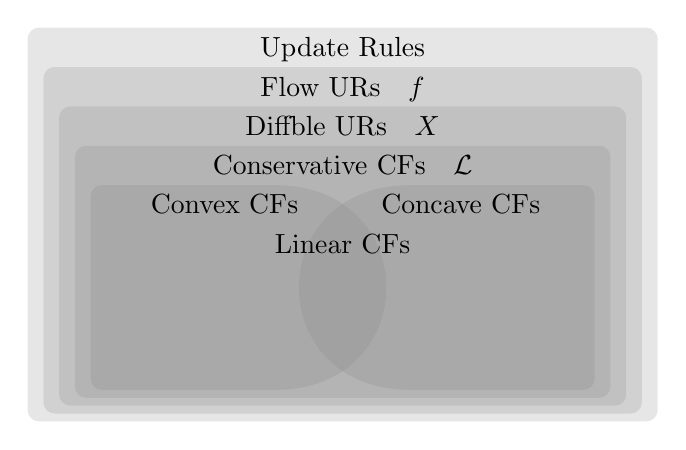
\begin{tikzpicture}
		\begin{scope}[fill=gray,fill opacity=0.2,rounded corners=4px]
			\fill (0,0) rectangle (8,5); % URs (Full Updates)
			\fill[] (0.2,0.1) rectangle (7.8,4.5); % Flow URs (Flows)
			\fill[] (0.4,0.2) rectangle (7.6,4.0); % Diffble URs (Vec Field)
			\fill[] (0.6,0.3) rectangle (7.4,3.5); % Conservative URs 
			\fill (0.8,0.4) -- (0.8, 3.0) -- (3, 3.0)
			 	to[out=0,in=0,looseness=2] (3,0.4) --cycle; % CONVEX
			\fill (7.2,0.4) -- (7.2, 3.0) -- (5, 3.0)
			 	to[out=180,in=180,looseness=2] (5,0.4) --cycle; % CONCAVE
		\end{scope}
		\begin{scope}[anchor=north]
			\node at (4.0, 5.0) {Update Rules};
			\node at (4.0, 4.5) {Flow URs~~~$f$};
			\node at (4.0, 4.0) {Diffble URs~~~$X$};
			% \node at (4.0, 3.5) {Conservative CFs~~~$\mathcal L$};
			\node at (4.0, 3.5) {Conservative CFs~~~$\mathcal L$};
			\node at (2.5, 3.0) {Convex CFs};
			\node at (4.0, 2.5) {Linear CFs};
			\node at (5.5, 3.0) {Concave CFs};
		\end{scope}
	\end{tikzpicture}
	\caption{%
		A map of different kinds of commitment functions and their representations.}
	\end{figure}
	}

\begin{figure*}
\centering
\begin{tikzpicture}
\begin{scope}[every node/.style={align=left,rounded corners=3,draw,thick,inner sep=5pt,anchor=center}]
	\node at (-5, 0) (fc) {Full-Confidence Update\\
		$(\,\cdot\mid \cdot\,) : \Theta \times \Phi \to \Theta$\\
			\small\hfill\color{gray}(idempotent)\hfill};
	\node at (0, -1.4)(flow) {Complete Positive Flows\\
		$f: [0,\infty] \times \Phi \times \Theta \to \Theta$\\
			\small\hfill\color{gray}(diffble, additive, limiting)\hfill};
	\node at (0, 1.4)(path) {Smoooth Paths\\ 
		$\gamma: [0,1] \times \Phi \times \Theta \to \Theta$\\
		\small\hfill\color{gray}(diffble, end-halting)\hfill};
	\node at (4.5, 0)(vfield) {Vector Fields \\
		$F : \Phi \to \mathfrak X(\Theta)$\\
		\small\hfill\color{gray}(complete, terminating)\hfill};
	\node at (8.5, 0) (loss) {Loss Repr \\
		$\mathcal L : \Theta \times \Phi \to \mathbb R$};
\end{scope}
	\draw[arr] (loss) to node[above]{$\hat\nabla$} (vfield);
%
	\draw[arr] (path) to[out=7,in=85] 
		node[right=5pt,pos=0.7]{$\frac{\partial}{\partial c}$} (vfield);
	\draw[arr] (flow) to[out=-7,in=-85]
		node[right=3pt,pos=0.7]{$\frac{\partial}{\partial t}$} (vfield);
%
	\draw[arr] (vfield) to[out=-95,in=-2] node[above=0pt,pos=0.75]
		% {$\int \mathrm dt$}
		% {$\int dt$} 
		{$\int$}
		(flow);
	% \draw[arr1] (vfield) to[out=90,in=0] node[below right]{$\int \mathrm dt$} (path);
	% \draw (vfield) to[out=90,in=0] node[above]{$\int \mathrm dt$} (flow);
	\draw[arr] (path) to node[above, sloped]{$\scriptstyle c=1$} (fc);
	\draw[arr] (flow) to node[below,sloped]{$\scriptstyle t=\infty$}(fc);
	
	\draw[arr,-left to,dotted,gray] (path) edge[transform canvas={xshift=4pt}] 
		node[right]{$\scriptstyle-\log(1-c)$} (flow);
	\draw[arr,-left to,dotted,gray] (flow) edge
	 	node[left]{$\scriptstyle1-e^{-t}$}(path);
	% \draw[arr,-left to] (path.south)++(0.1,0) to (flow.north)+(0.1,0);
	% \draw[arr,-left to] (flow.north) to (path.south);
\end{tikzpicture}
\caption{Different representations of update functions, and the relationships they have with one another. 
Sections 3 and }\label{fig:map}
\end{figure*}


\begin{example}\label{ex:jugo}
% \def\Gpressed(#1,#2){\mathsf{G}_{#1}\text{-}\mathit{pressed}(\mathsf{G},#1,#2)}
% \def\Gpressed(#1,#2){\mathit{pressed}(#1,\mathsf{G},#2)}
\def\pressed(#1,#2,#3){\mathit{pressed}(#1,\mathsf{#2},#3)}
Jugo is an impartial juror.
Like the other jurors, she has two buttons in front of her,
labeled $\sf G$ and $\sf N$.
% The button labeled $\mathsf G$ increases the probability 
% of a guilty verdict, while the button labeled $\mathsf N$ increases
% the probability of a not-guilty verdict. 
Her instructions are to listen to evidence, and press $\sf G$ to 
increase the probability of a guilty verdict, and $\sf N$ 
to increase the probability of a not-guilty verdict.

More concretely, the system works as follows.
There are $J$ jurors, labeled $\{1, \ldots, J\}$;
let 
% $G_j(t)$ be
$\pressed(j,B,t)$ be
a variable that is equal to one if juror $j \in $
is pressing button  $\mathsf B$ button at time $t$, and zero otherwise.
% ; symmetrically, let $N_j(t)$ indicate whether $j$ is pressing the $\mathsf N$ at time $t$.
The ``belief state'' of this automated system is
a single number $g \in [0,1]$, representing the probability of a guilty verdict.
When a single juror presses $\mathsf G$, $g$ approaches 1
exponentially, and if they instead press $\sf N$, $g$ decays to zero.
In the first case ($\sf G$ is pressed) the system evoves according to 
$\frac{\mathrm dg}{\mathrm dt} = (1-g)$
while in the second, 
$\frac{\mathrm dg}{\mathrm dt} = -g$.
The first is the vector field associated with the $\mathsf G$ button,
and the second is the vector field associated with $\sf N$. 
The total effect of all buttons is then the sum of that of all buttons across all vector fields, when they are active:
% in which case $g(t) = 1 + (g(0) - 1)e^{-t} $.
% Concretely, their dynamics are governed by:
\[
	\frac{\mathrm dg}{\mathrm dt} = 
	\sum_{j = 1}^J 
		% G_j(t)
		\pressed(j,G,t)
		(1-g) 
		-
		% N_j(t)
		\pressed(j,N,t)
		(g)
		~,
	% \begin{cases}
	% 	(1 - p)	& \text{button $\uparrow$ pressed} \\
	% 	-p & \text{button $\downarrow$ pressed}
	% \end{cases}	
\]
so that $g$ exponentially approahces $1$ when more $\mathsf G$ buttons are pressed than $\mathsf N$ buttons,
and symmetricaly, exponentially approaches $0$ when more $\mathsf N$ buttons than $\mathsf G$ buttons are pressed.
At the end of the trial, the defendant is convicted with probability
equal to the final value of $g$. 

Let $\phi$ represent a piece of evidence suggesting guilt, presented by the
prosecution from time $t_1$ to time $t_2$,
and suppose for now that only buttons labeled $\mathsf G$ are pressed
in this interval.
% Many aspects of this scenario can be understood in terms of confidence.
%
	% The amount of time that 
	% What is the confidence of the system in that evidence, as it understands it from the Jurors?
% First, suppose that only $\mathsf G$ buttons are pressed
	 % between $t_1$ and $t_2$. 
% in between times $t_1$ and $t_2$.
The system measures $j$'s confidence in $\phi$ by
\[
	w_j := \!\int_{t_1}^{t_2}\!\! G_j(t) \mathrm d t 
	= \text{ total time $j$ presses $\mathsf G$ during $\phi$,}
\]
Note that $w_j = 0$ if and only if $j$ does not press any buttons,
which (a) indicates that $j$ does not trust the evidence $\phi$, 
and (b) communicates this fact to the system, by telling it to ignore 
the evidence. 
Note that this is an additive representation of confidence, since
pressing the button for four seconds, and then three more later, is
by definition the same as pressing it for seven. 
While the maximum possible confidence of $w_j$ is $(t_2 - t_1)$,
this system does not allow a juror to express \emph{full} confidence in $\phi$
because no finite amount of $\mathsf G$-pressing will result in a 
guilty verdict with probability one; it is always possible to increase
the value of $g$ through additional evidence. 

% Now, recall that ,
Altogether, the system's confidence in $\phi$ can be measured by
as the unique value $W$ for which
\begin{align*}
	% \int_{t_1}^{t_2} W (1-g(t)) \mathrm d t = \int_{t_1}^{t_2} \sum_{j=1}^J G_j(t) (1-g(t)) \mathrm d t,
	\int_{t_1}^{t_2} W (1-g(t)) \mathrm d t =
	 g(t_2) - g(t_1),
	% \\
	% W = \frac{1}{t_2-t_1 - \int_{t_1}^{t_2}g(t) \mathrm dt} \int_{t_1}^{t_2} \sum_{j=1}^J G_j(t) (1-g(t)) \mathrm d t
\end{align*}
which, so long as only $\mathsf G$ buttons are pressed, equals
$W := \sum_{j} w_j$, so this measure of confidence is additive 
across jurors as well as across time. 
This is appropriate, since the jurors are independent and 
not communicating with each other.
% This is a weighted sum of $w_i's$
As before, $W = 0$ if and only if no juror presses any buttons between times $t_1$ and $t_2$,
indicating zero trust leant to $\phi$. In such a case, the system ignores $\phi$ in updating its beliefs.
And just as no individual juror can send a full-confidence update to the system,
	the system cannot recieve a full-confidence from the jurors as a whole.
	
The picture gets significantly more complicated if we consider the possibility
that jurors might press the $\mathsf N$ button. For example, if $\phi$, which was intended
as evidence of guilt, has the effect of getting jurors to press $\mathsf N$, there is a sense
in which they have \emph{negative} confidence in $\phi$, since the belief update happened in the opposite direction of what $\phi$ represents; rather than \emph{no} trust, this is represents \emph{distrust}. 
Small negative updates are always possible except at the boundary of belief space, but in this paper, we focus almost entirely on positive confidence updates.

The introduction of the second button also uncovers a significant source of complexity:
unlike \cref{ex:prob-simple,ex:classifier,ex:shafer}, 
the order that evidence is presented matters, when there is more than one possible response to it.
Evidence presented later has a larger effect,
meaning that this system exhibits a recency bias.
% (This lack of commutativity corresponds to possibility that,
%	as a Lie algebra, the bracket may not be identically zero.)

Now consider a variant of this system that does
not trust all jurors equally; rather, it trusts each juror $j$
to a degree $\beta_j \in [0, \infty]$, and now $g$ evolves
according to
\[
	\frac{\mathrm dg}{\mathrm dt} = 
	\sum_{j = 1}^J \beta_j \Big( G_j(t) (1-g) 
		- g N_j(t) \Big).
	% \begin{cases}
	% 	(1 - p)	& \text{button $\uparrow$ pressed} \\
	% 	-p & \text{button $\downarrow$ pressed}
	% \end{cases}	
\]
In this case, the system can be said to have trust $\beta_j$ in juror
$j$, since $j$'s buttons are ignored when $\beta_j = 0$. 
When $\beta_j = \infty$ (an expression of full confidence in $j$),
$g$ immediately jumps to 0 when $j$ presses 
$\mathsf N$, or to 1 if $j$ presses $\mathsf G$ (unless canceled by
another full-confidence juror pressing the opposite button).
If all jurors have full confidence, then the verdict of this system is
a majority vote at the last moment a button was pressed. 
Thus, the weights attached to weighted combinations are (additive) expressions 
of confidence as well. 
\end{example}

\cref{ex:jugo} illustrates how a (sufficiently nice) vector field, 
	which is simpler than a smooth path for every starting point, is enough to define
an additive notion of confidence, via its integral curves.
It may seem strange to define confidence via a vector field, which does not mention confidence at all---but in a sense, it works because a vector field captures precisely everything about the update \emph{except} for the confidence. We do this formally in \cref{sec:vecrep}. 

In \cref{sec:loss-repr}, we demonstrate that it is typically possible to get an even more compact representation of the updating process, by representing the vector field implicitly as gradients of some ``loss function''.
To do this at full generality, we need to make sense of a gradient, which requires more structure, in the form of a Riemannian metric.  It turns out that, up to a multiplicative constant, there is a unique natural Riemannian metric on any parameterization of a probability distributions \cite{chentsov}; taking gradients with respect to this geometry, show how familiar loss functions on probability measures correspond to different standard notions of confidence in the other representations.

Once we have the formalism, fully in place, we give further examples of how confidence works in exponential families, in particular showing how Kalman gain and inverse variance can be viewed as confidence as well.
% Say 


\commentout{
This general idea can be cleaned up by appeal to differential geometry.
Fix an input $\phi$.
Assuming that the update paths are differentiable in the degree of confidence at any initial beleifs, the collection of updates with infinitessimal confidence forms a complete vector field $X_\phi$ over the space of beliefs, whose integral curves are paths in belief space, parameterized by confidence $\beta \in [0,\infty]$.
% Of course, we may always convert this number back to $[0,1]$,
We step through this more carefully in \cref{sec:field-repr}.

%joe1*: NO!  This is not the place to bring up Reimannian metrics!
Finally, if our belief space is endowed with a Riemannian metric, so that we may take gradients, partial update functions may be specified by a loss.}


% natural measure of confidence that works in all cases,
% which 
% It turns out that there is a natural way of measuring confidence in all cases of interest, based on differential geometry of belief space. 
% Furthermore, in the case where belief states are Dempster-Shafer belief functions, 
% and inputs are simple support functions, this measure of confidence is what Shafer calls the ``weight of evidence''.
%% TODO: Shafer



% It is not always most natural for confidence to range between zero and one. 
% But there are many instances in which 
% However, there is a more universal representation of it in $[0, \infty]$

% While probability ranges from untenable (0) to undeniable (1),
% confidence ranges from completely untrustworthy $(\bot)$ to fully trusted ($\top$).




\commentout{
	\subsection{Other Conceptions of Confidence.}

	\textbf{Probability.}
	% Probability is a numerical scale that ranges from untenable (0) to undeniable (1).
	% No number on this scale is truly neutral.
	% One of the biggest shortcomings of probability is its inability to represent a truly neutral attitude towards a proposition.
	Some people do use ``confidence'' to mean the same thing as probability. When they say they have low confidence in $\phi$, they mean that they think $\phi$ is unlikely.

	One of the biggest shortcomings of probability is its inability to represent a truly neutral attitude towards a proposition.
	%  probability of $\frac12$ .
	% This shortcoming has perhaps been the primary selling point of many alternatives to probabiltiy, such as Dempster-Shafer Belief functions.
	A value of $\frac12$ may be equally far from zero as it is from one, but is by no means a neutral assessment in all cases: hearing that your favored candidate has a 50\% chance of winning is big news if a win was previously thought to be inevitable.
	For this reason, telling someone the odds are 50/50 is quite different from saying you have no idea.
	% By contrast, zero confidence represents a truly neutral stance; a statement with zero confidence has no effect.
	By contrast, zero confidence represents something truly neutral:
		a statement made with zero confidence does not stake out a claim, and
		a statement recieved with zero confidence does not affect the recipient's beliefs.
	Nevertheless, in some contexts, we will see that confidences correspond to to probabilities.

	\textit{Opacity.} To use a graphical metaphor, think of certainty as black or white.
	Probability describes shades of gray, while confidence describes opacity.
	If we are painting with black and start with a white canvas, there is a precise correspondence between the opacity and the resulting shade of gray.

	\textbf{Upper and Lower Probabilities.}
	Upper and lower probabilities can describe a neutral attitude towards a proposition, but they are not really a specification of trust, but rather a direct specification of a belief state.
	It isn't immediately clear how to use these representations of uncertainty to update, and they're a little too complex to function effectively as the primitive measure of trust that we're after.


	\textbf{Shafer's Weight of Evidence.}
	Shafer's ``weight of evidence'' is precisely the same concept we have in mind.
	Our analysis precsely reduces to his, in the setting where belief states are Belief functions (which generalize probabilities, but not, say, neural network weights), and observations are events.
	% This paper can be a generalization of Shafer's ``weight of evidence'' to a broader class of settings, where one might have very different belief states and observations.
	Thus, this paper can be viewed as generalizing this concept to a broader class of settings, without requiring that one adopt Shafer's conception of a belief state or an observation.


	\textbf{Variance and Entropy.}
	The inverse of variance, sometimes known as precision,
		is also commonly used to measure confidence.
	If a sensor is unreliable and can give a range of answers, the variance of the estimate is a very common way of quantifying this reliablility.
	If measurements have zero variance, in some sense one has absolute confidence ($\top$) in the sensor. If measurements have infinite variance, then in some sense one has no confidence in the sensor, since individual samples convey no information about the true value of the quantity measured.
	As with probability, inverse variance will coincide with confidence in some settings; we will see how in \cref{sec:variance}.

	Entropy, like variance, is a standard way of measuring uncertainty, and in some settings, confidence coincides with entropy (see \cref{sec:entropy}).
	The assumption underlying both approaches is that there's some ``true'' value of the variable, and that the randomness is epsistemic (due to sensor errors) rather than aleotoric (inherrent in the quantity being measured).

	\textbf{Confidence Intervals and Error Bars.}
	Another notion of the word ``confidence'' comes from the term ``confidence interval''.
	This concept arises in settings involving a probability distribution $\Pr(X)$ over a metric space $X$, typically $X = \mathbb R$.
	A 95\% confidence interval is the (largest) ball containing 95\% of the probability, and its size is a geometric measurement of how .
	This intuition behind this reading of the word confidence is the same as
}
